\documentclass[a4paper, 12pt]{article}

\usepackage[english, russian]{babel}
\usepackage[T2A]{fontenc}
\usepackage[utf8]{inputenc}
\usepackage{mathtext}
\usepackage{amsfonts}
\usepackage{ amssymb }
\usepackage{amsmath}
\usepackage{graphics}
\usepackage{graphicx}
\usepackage{wrapfig}
\usepackage{geometry}
\usepackage{float}
\geometry{
	a4paper,
	total={170mm, 257mm},
	left=20mm,
	top=10mm}

\date{\today}
\author{Абакшин Василий, Б05-207}
\title{Лабораторная работа 3.4.1. Диа- и парамагнетики}

\begin{document}
	\maketitle
	\section*{Краткие теоретические сведения}
	Измерение магнитной восприимчивости материалов будем проводить с помощью расчета силы, действующей на магнетик в магнитном поле. При смещении образца на расстояние $ \Delta l $ внутрь магнитного поля магнитная сила, действующая на него, равна
	
	\begin{equation}
		F = \left(\frac{\Delta W_m}{\Delta l}\right)_I,
	\end{equation}
	где $ \Delta W_m $ -- изменение магнитной энергии системы при постоянном токе
	в обмотке электромагнита и, следовательно, при постоянной величине
	магнитного поля в зазоре.\\
	Магнитная энергия рассчитывается по формуле:
	\[W_m=\frac{1}{2}\int (\mathbf{H}\mathbf{B})d\,V = \frac{1}{2\mu_0}\int\frac{B^2}{\mu}d\,V,\]
	\begin{wrapfigure}[10]{l}{0.3\textwidth}
		\centering
		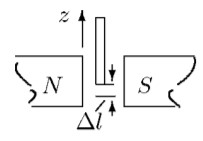
\includegraphics[height = 0.12\textheight]{energy}
		\caption{Перемещение магнетика}
	\end{wrapfigure}
	

	 При смещении образца магнитная энергия меняется только в области зазора (в объёме площади $ S $ и высоты $ \Delta l $), а около верхнего конца стержня остаётся неизменной, поскольку магнитного поля там практически нет. Тогда изменение магнитной энергии будет:
	\[\Delta W_m=\frac{1}{2\mu_0}\frac{(\mu B)^2}{\mu}S\Delta l - \frac{1}{2\mu_0}B^2 S\Delta l = (\mu - 1) \frac{B^2}{2\mu_0}S\Delta l \]
	
	Следовательно, на образец действует сила
	\[F = (\mu - 1)\frac{B^2}{2\mu_0}S = \chi\frac{B^2}{2\mu_0}S\]
	
	Знак силы, действующей на образец, зависит от знака $ \chi $: образцы из парамагнитных материалов $( \chi  > 0)$ втягиваются в зазор электромагнита, а диамагнитные образцы $ (\chi < 0) $ выталкиваются из него.
	
	\section*{Экспериментальная установка}
	
	\begin{figure}
		\centering
		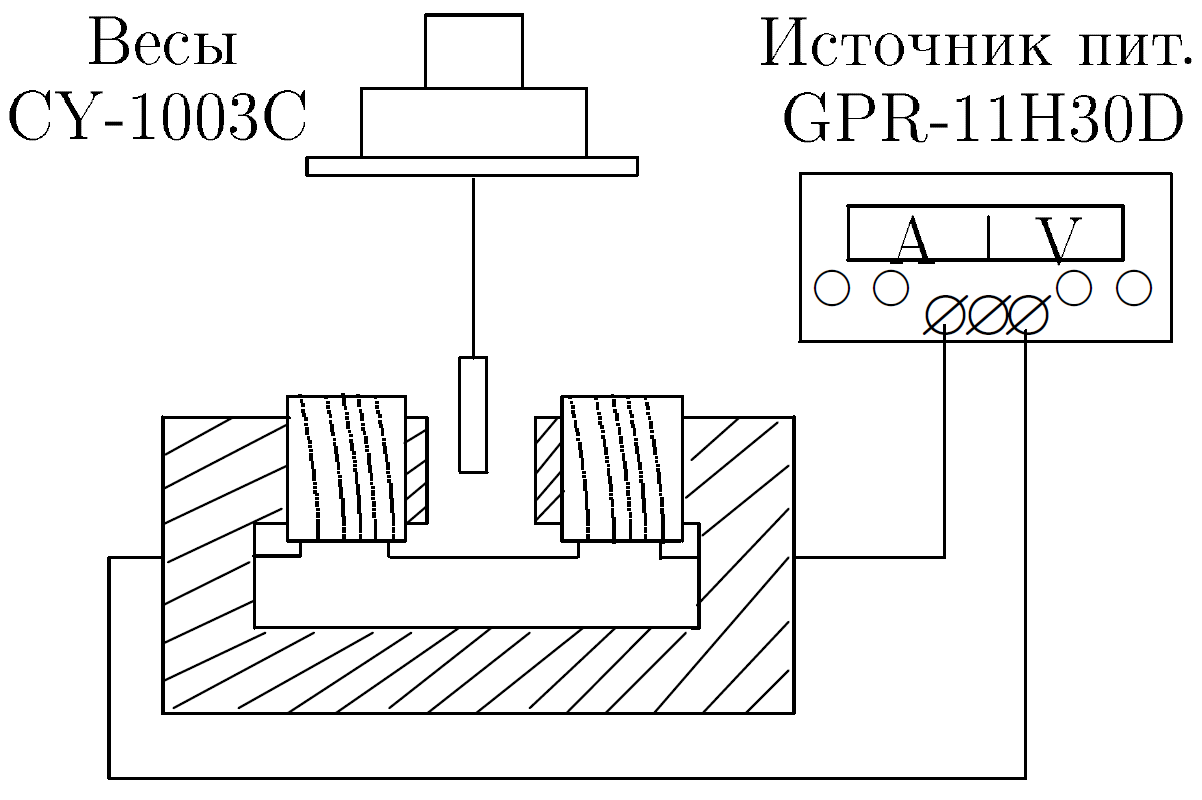
\includegraphics[width = 0.7\textwidth, height = 0.3\textheight]{ustanovka}
		\caption{Схема экспериментальной установки.}
	\end{figure}
	
	
	Магнитное поле создаётся в зазоре электромагнита, питаемого постоянным током. Диаметр полюсов существенно превосходит ширину зазора, поэтому поле в средней части зазора однородно. Величина тока, проходящего через обмотки электромагнита, задаётся регулируемым источником питания GPR и измеряется амперметром $ А $, встроенным в источник питания. Градуировка электромагнита (связь между индукцией магнитного поля $ B $ в зазоре электромагнита и силой тока $ I $ в его обмотках) производится при помощи милливеберметра либо тесламетра.\\
	Сила, действующая на образец со стороны магнитного поля измеряется в помощью весов: смотрится разность веса образца вне поля и в поле.
	
	\section*{Ход работы}
	
	\subsection*{Градуировка электромагнита}
	
	Сначала проведём градуировку магнита: с помощью тесламетра измеряем магнитное поле при разных токах:
	
	\begin{table}[H]
		\centering
		\begin{tabular}{|c|c|c|c|c|c|c|c|c|}
			\hline
			$ I $, А   & 0,22   & 0,30   & 0,45   & 0,60   & 0,75   & 0,90   & 1,05   & 1,15 \\ \hline
			$ B $, мТл & 236,2 & 300,2 & 448,8 & 598,8 & 733,5 & 933,2 & 1103,2 & 1144,7 \\ \hline 
		\end{tabular}
		\caption{Результаты измерений}
	\end{table}
	
	По полученным данным построим график зависимости $ B(I)$.
	
	\begin{figure}[h!]
		\centering
		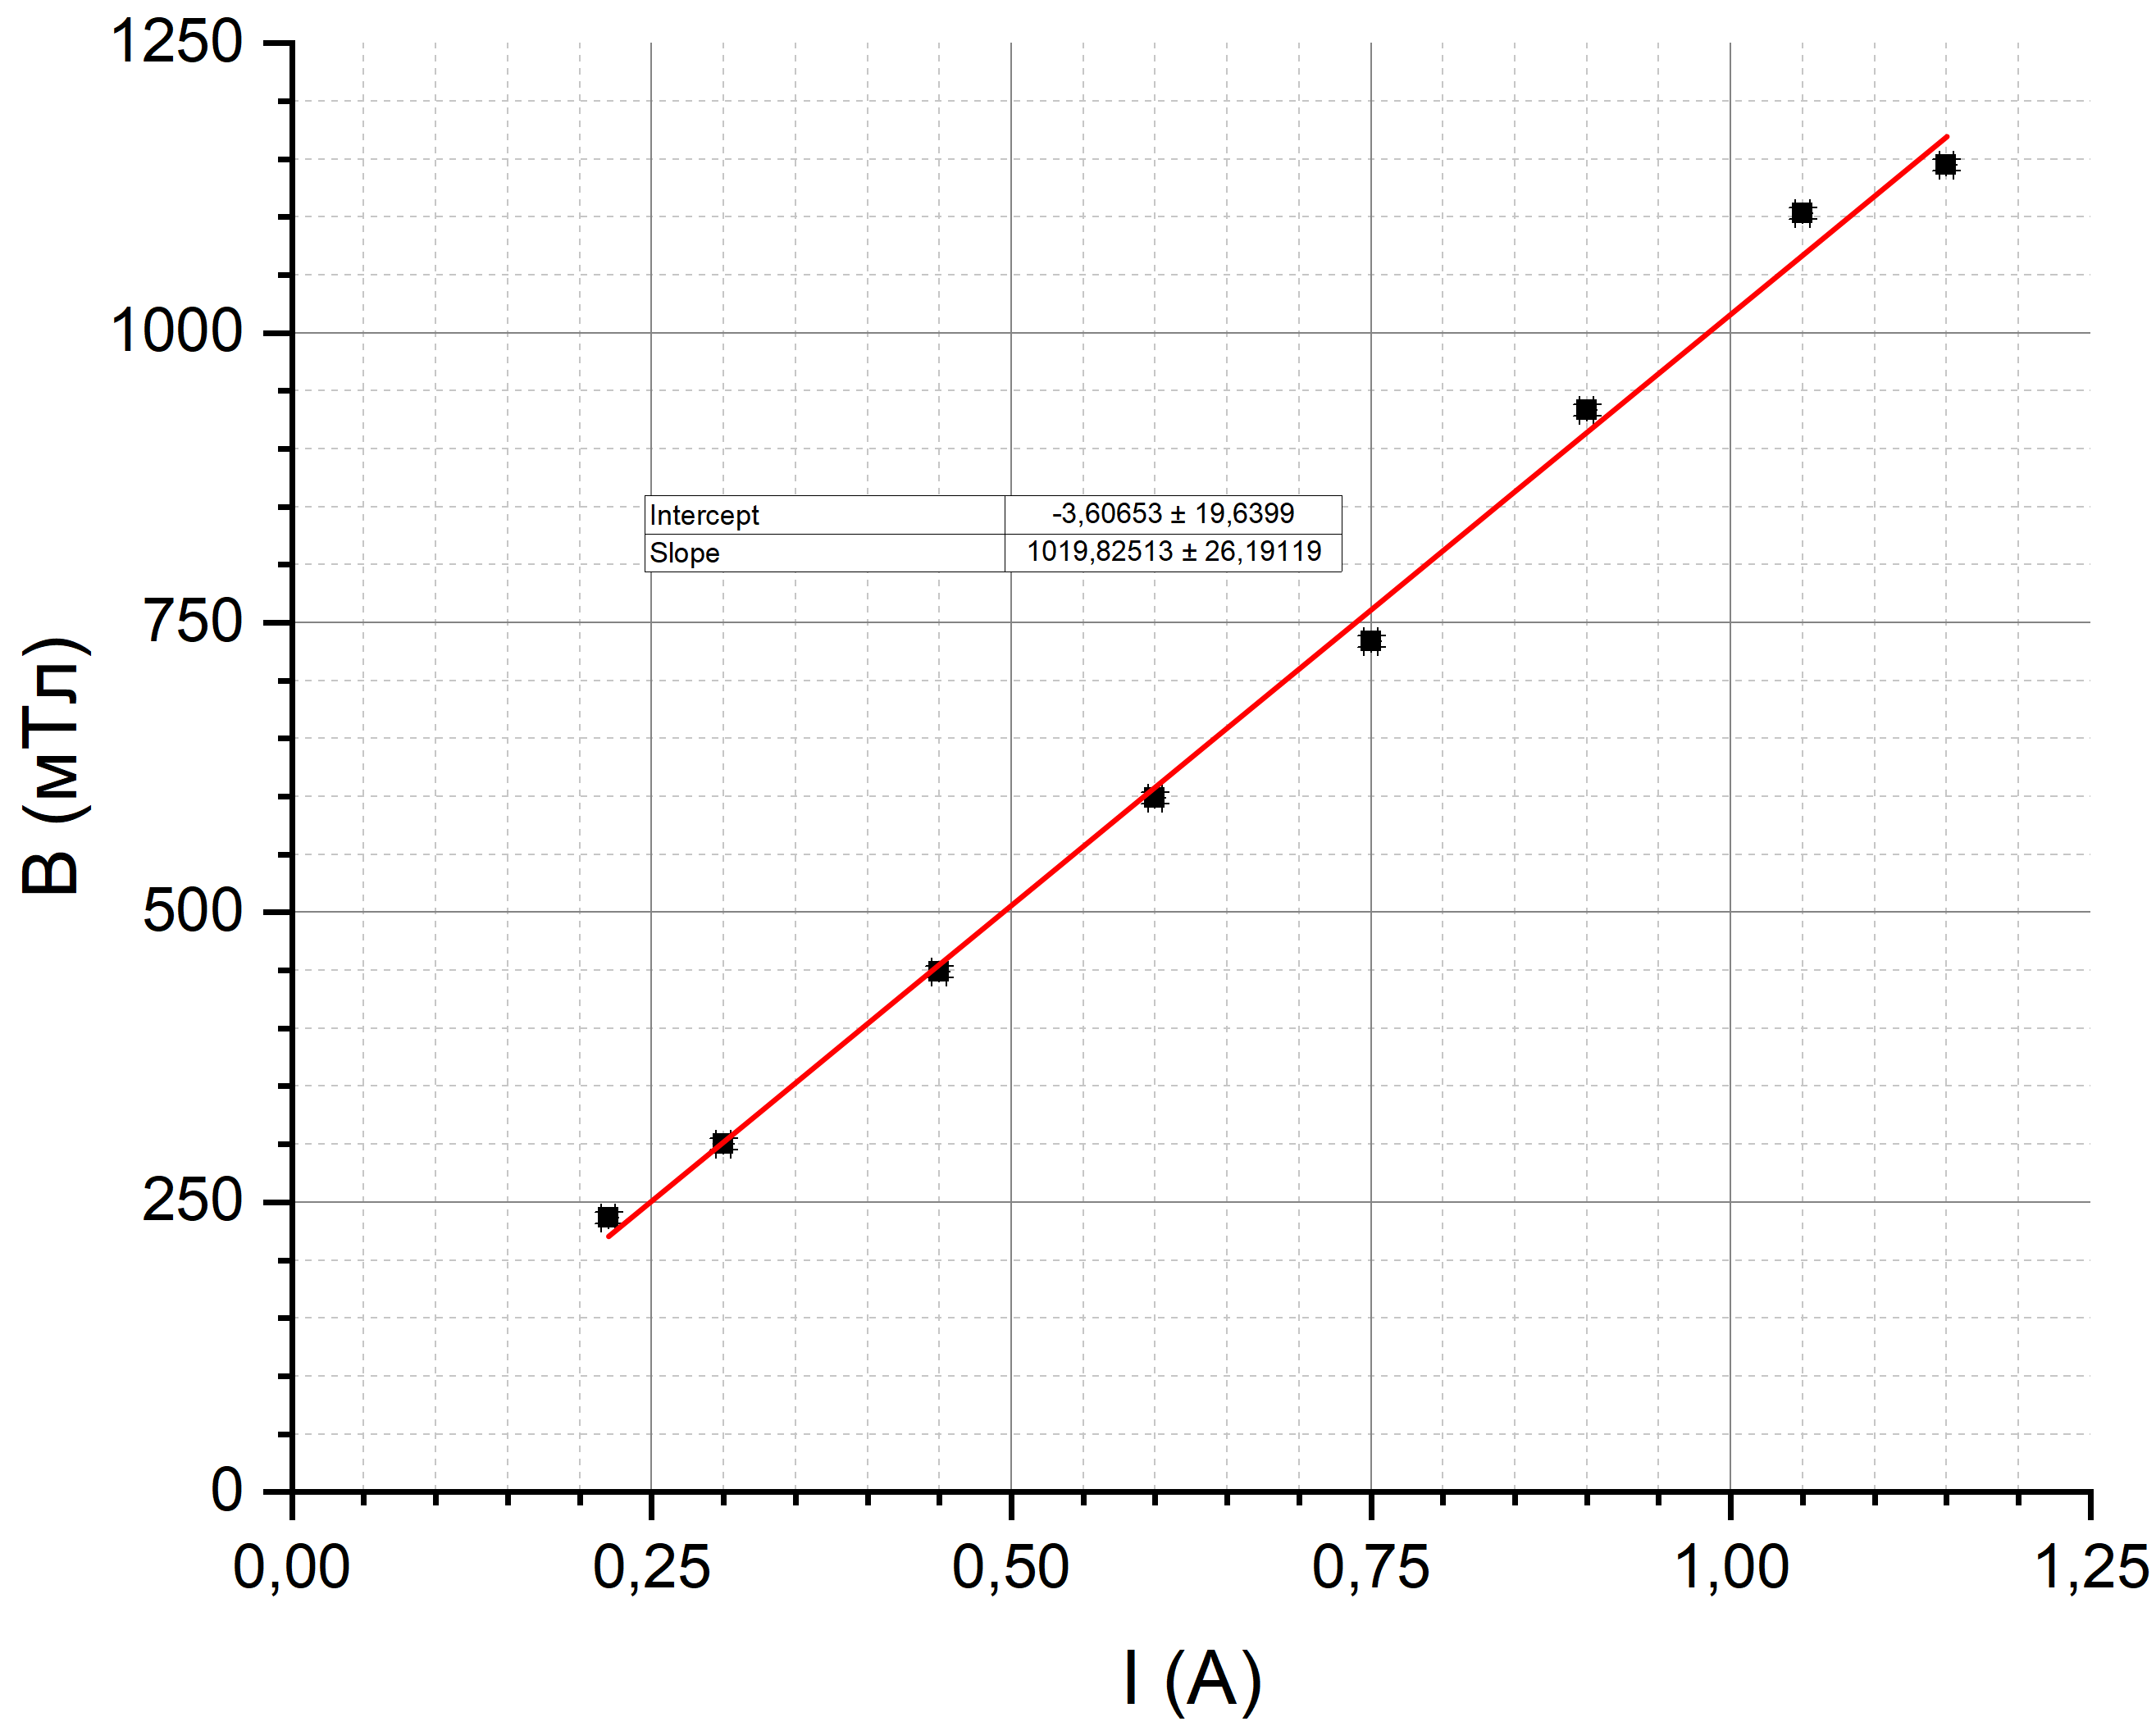
\includegraphics[width = \textwidth]{Graduation}
		\caption{Градуировка электромагнита $B(I)$}
	\end{figure}
	
	\subsection*{Измерение сил, действующих на образцы в магнитном поле}
	
	При нулевом токе через электромагнит подвесим к весам один из образцов так, чтобы он не касался наконечников электромагнита. Обнулим показания весов, чтобы измерять непосредственно перегрузки $ \Delta P = F $ -- силы, действующей на образец при различных токах в обмотках электромагнита. Были получены следующие значения:\\
	$m_{Al} = 25,228$ г, $m_{Cu} = 83,270$ г, $d = 1 \pm 0,01$ см (диаметр образцов). 
	\begin{table}[h!]
		\centering
		\begin{tabular}{|c|c|c|c|c|c|c|c|c|}
			\hline
			$I$, A & 0,22 & 0,30 & 0,45 & 0,60 & 0,75 & 0,90 & 1,05 & 1,15 \\ \hline
			Al, $\Delta m$, мг & 4 & 7 & 15 & 24 & 36 & 49 & 62 & 70 \\ \hline
			Cu, $\Delta m$, мг & -3 & -4 & -7 & -12 & -17 & -23 & -29 & -32 \\ \hline
		\end{tabular}
		\caption{Изменение веса образцов в магнитном поле}
	\end{table}
	
	\begin{figure}[h!]
		\centering
		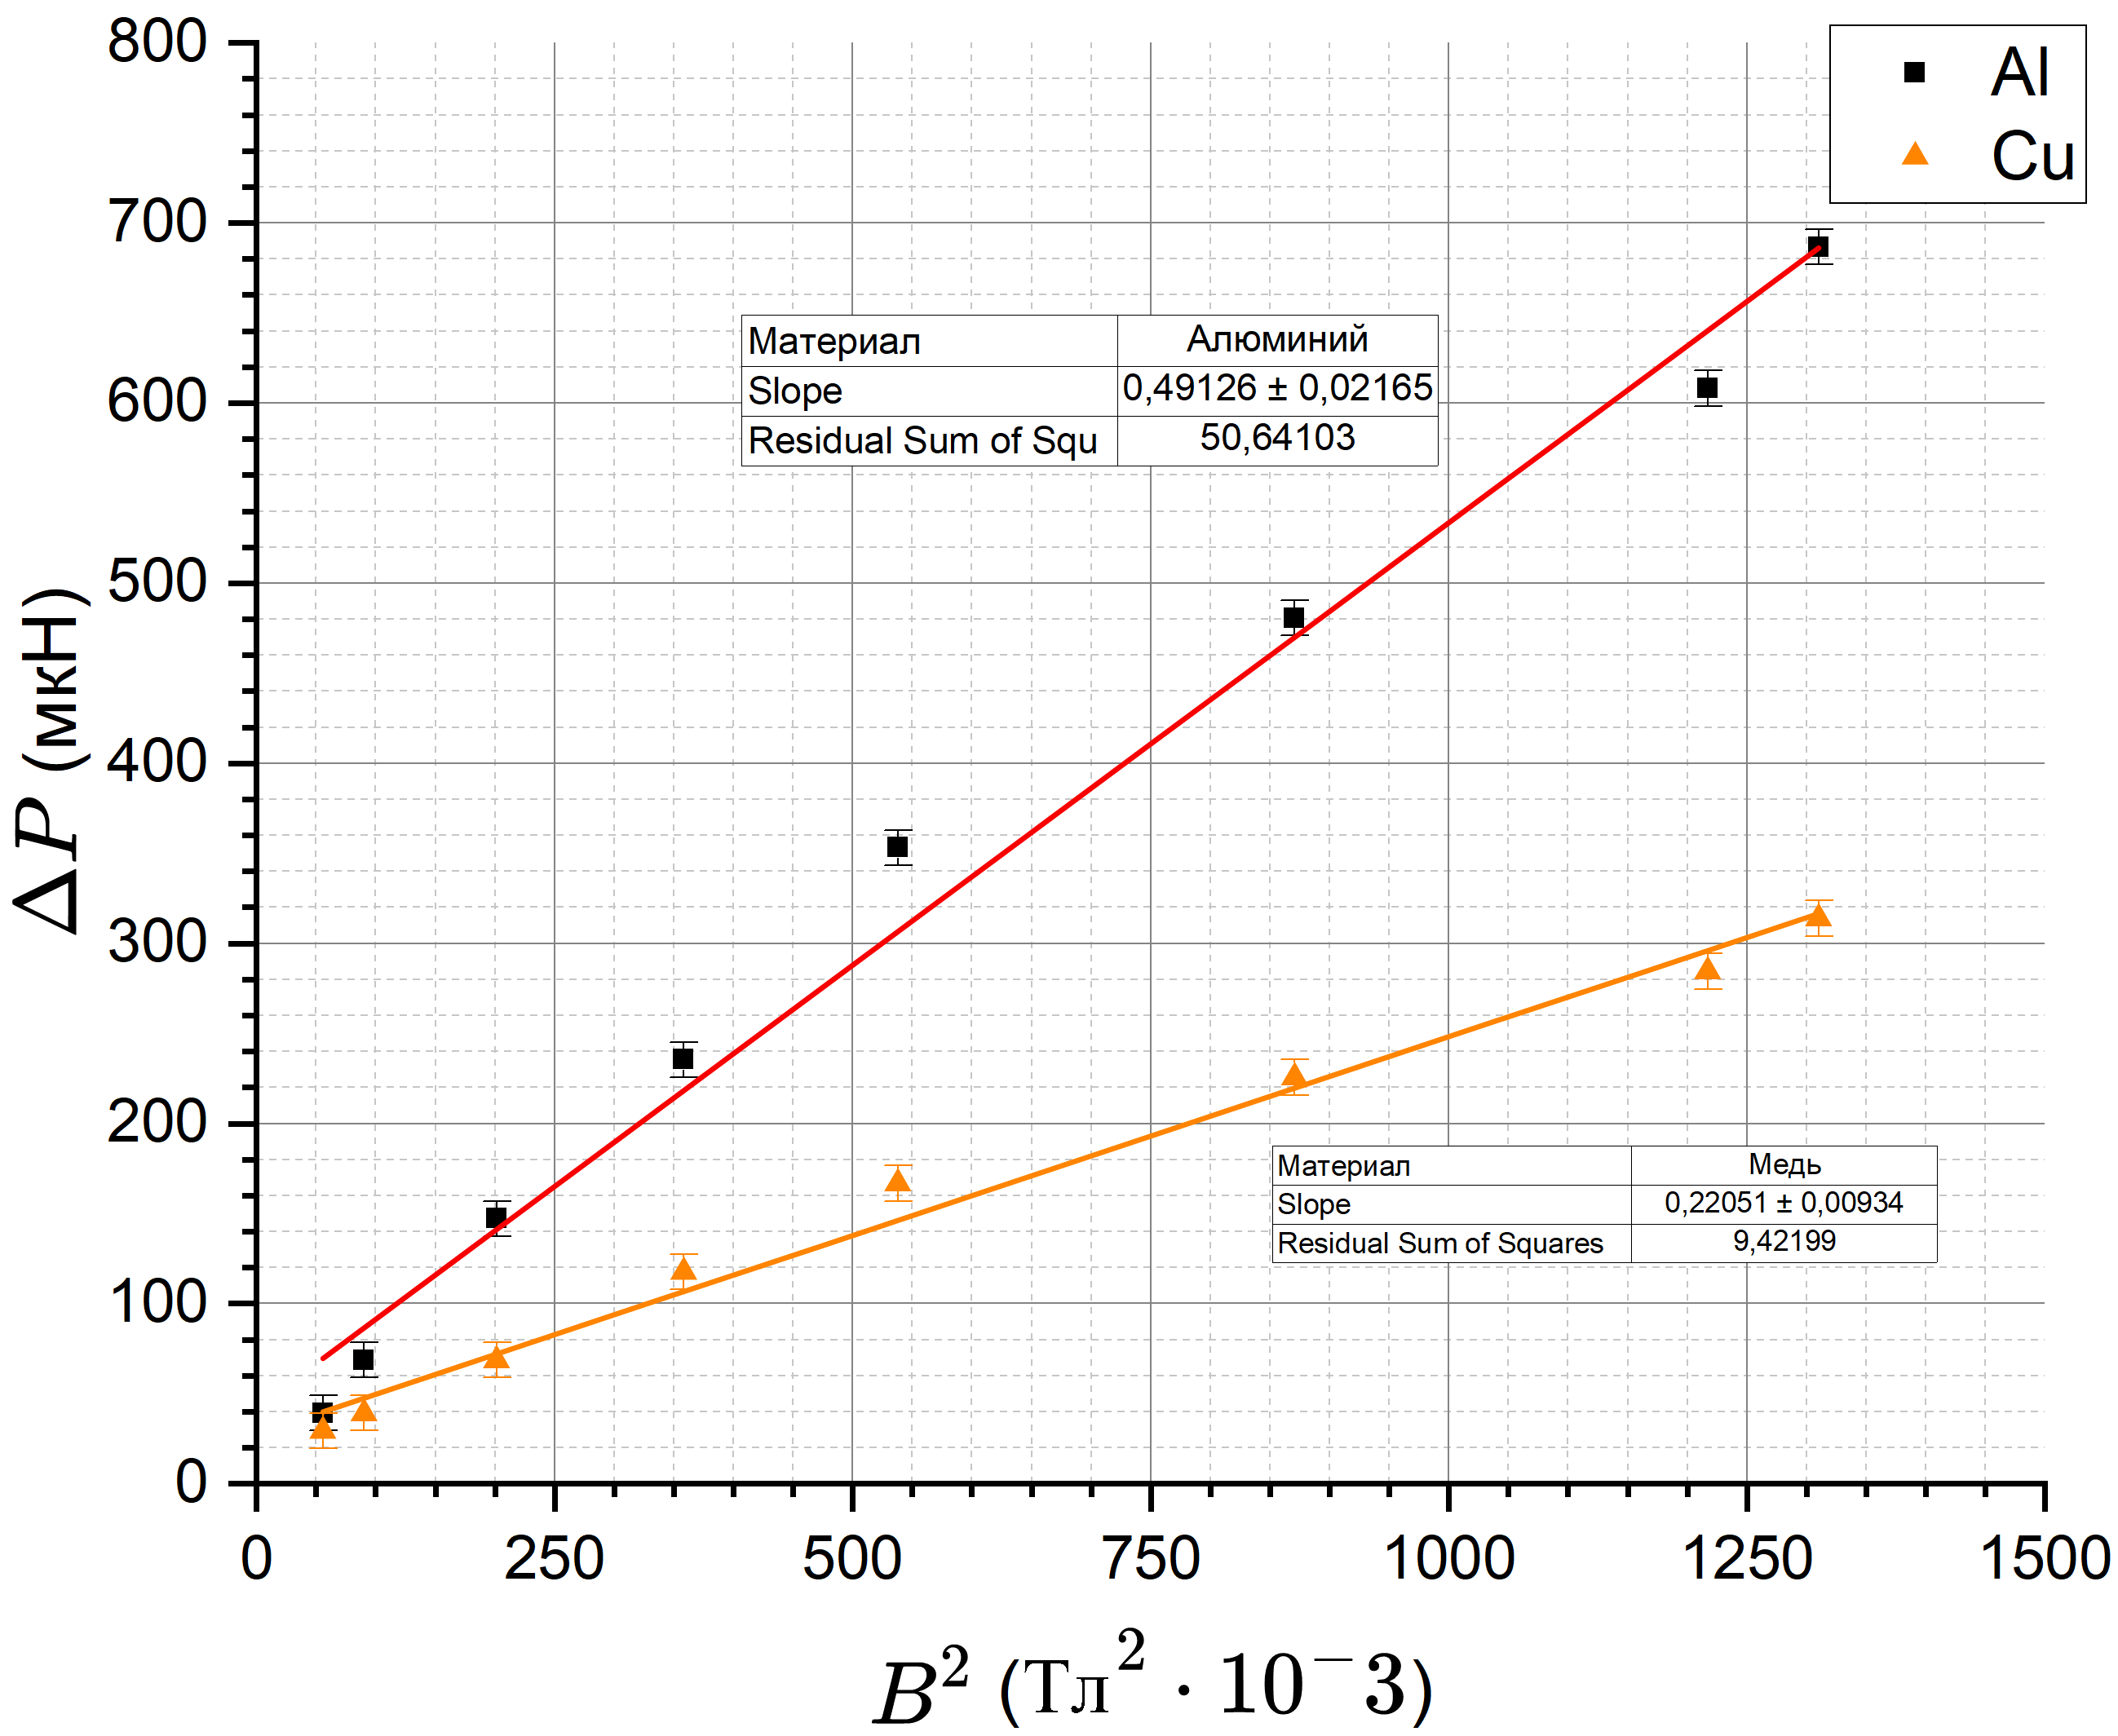
\includegraphics[width = \textwidth]{Main}
		\caption{Зависимость $\Delta P(B^2)$}
	\end{figure}

	\subsection*{Расчёт магнитной восприимчивости}
	Построим графики зависимости $\Delta P(B^2)$ для меди и алюминия. Если $k$ - угловой коэффициент наклона графика, то
	\[k = \frac{\chi S}{2\mu_0} \ \rightarrow \chi = \frac{2\mu_0 k}{S}\]
	где $ S $ -- площадь поперечного сечения исследуемых образцов. В нашем случае $ S = (0,785 \pm 0,016) $ см$ ^2 $ для всех образцов.
	Для меди значения для графика были взяты по модулю чисто для расчета, сам коэффициент будет отрицательным. Полученные значения представлены в таблице.

	
	\begin{table}[h!]
		\centering
		\begin{tabular}{|c|c|c|c|}
			\hline
			Материал & $k$ & $\chi$ & $\varepsilon_{\chi}$ \\ \hline
			Алюминий Al & $0,491 \pm 0,022$ & $(15,72 \pm 0,79) \cdot 10^{-6}$ & 4,9\% \\ \hline
			Медь Cu & $0,221 \pm 0,009$ & $-(7,08 \pm 0,33) \cdot 10^{-6}$ & 4,7\% \\ \hline
		\end{tabular}
	\end{table}
	\newpage
	\section*{Выводы}
	
	В ходе данной работы была измерена магнитная восприимчивость образцов меди и алюминия. Для алюминия и меди табличные значения удельной магнитной восприимчивости равны $ \chi_{Al.\text{уд}} = 0,61\cdot 10^{-9} \ \frac{\text{м}^3}{\text{кг}}$ и $ \chi_{Cu.\text{уд}} = -0,086 \cdot 10^{-9} \ \frac{\text{м}^3}{\text{кг}} $ соответственно, получается $\chi_{Al} = 1,64 \cdot 10^{-6}$ и $\chi_{Cu} = -0,77 \cdot 10^{-6}$. Полученные экспериментально данные, к сожалению, на порядок не совпадают с табличными. Вероятно, это связано с наличием ферромагнитных примесей в экспериментальных образцах, так как даже очень малое их количество может привести к резкому возрастанию магнитной проницаемости.
	
\end{document}